\chapter{PID Controller Design}

\section{PID Controller Tuning}
The appropriate selection of the tuning parameters is one of the most important steps in the definition of a PID based control loop. This is known as the PID tuning. The selection of the PID controller parameters should be made according to the available knowledge of the process dynamics and stated performance specifications in terms of tracking and disturbance attenuation as well as desired robustness. One of the aspects that makes PID control specially appealing is the clear physical meaning associated to each one of its parameters. \\

Numerous studies have been made to develop assignment rules to specify PID parameters on the basis of characteristics of the process being controlled. The collected information about the process to be controlled can, in one form or another be assimilated to a model of the process. This can be referred either as a parametric process model (or, in other words, a form suitable for analyzing and simulating the closed-loop system), or concrete process data and/or measurements that in a suitable way can be directly employed to determine the PID controller parameters. There are many representative sources that can be consulted for details on a wide variety of alternative tuning rules  \cite{odwyer2006}, \cite{vilanova2012}. \\

In what follows, a short presentation of the most usual existing methods for PID tuning are presented. The presentation will not be deep into details because it is not the purpose of this book to explore existing tuning approaches, material that, on the other hand, can be accessed on numerous sources.  However, it is important not to forget the existing panorama and main features of existing approaches, This will make possible, in the next section, to better understand the formulation of the PID tuning problem as a multiobjective optimization problem.

\subsection{Analytical Tuning Methods}

These approaches allow a specification of a desired closed-loop time response. This desired closed-loop behavior can take the form of desired poles for the closed-loop behavior, or a reference model the closed-loop system should try to mimic.  These approaches were originated by the early works on algebraic controller design (of course in a more generic setting, not just for PID controllers) by \cite{ragazzini1958}. There are different approaches for doing that; some of them place only the closed loop poles, others also shape the zeros. In contrast, by using conventional PID controller, it may not be possible to place all of the poles, so only the dominant pole is placed for this scenario. The design notion in this class of designs is based on re-assigning the system's poles with faster modes. The drawback, however, is that some modes may become uncontrollable due to pole/zero cancellation and the performance degrades if they become excited.


The introduction of ideas on algebraic design, gave rise to the so called \emph{$\lambda$-tuning} or  Dahlin method \cite{dahlin68}. It is straightforward to see that for FOPTD and  SOPTD models, PI and PID
controllers can help achieve the desired performance. The number of poles that can be placed is equal to the number of controller parameters. Therefore these techniques can be used for process models with the maximum order of 2 if a PID controller is selected. This method, in turn, is closely related to the Smith predictor and the design method based on Internal Model Control (IMC) \cite{riveraetall86}.  It is worth a special mention the fact that, for a FOPTD process, the IMC controller takes the form of a PI or a PID controller depending on the rational approximation used for the time delay.  These approaches, however, use cancellation of the poles of the process, which may lead to quite undesirable responses to load disturbances, especially for processes with very large time constants. In \cite{chien90} a modification is presented  that does not cancel the poles of the process, while \cite{skogestad2003}, presents a variation of the IMC controller, applied to PI and PID controller tuning, denominated SIMC, in which the cancellation is avoided by means of a redefinition of the integral mode for the cases of systems dominated by large time constants. 

In 2002,  Lee and Seborg,\cite{chenseborg2002} proposed a modification of the direct synthesis method adapted to disturbance rejection instead of set-point change. Tuning rules are provided for a wide range of process models. Following these lines, in 2007  Shamsuzzoha and Lee \cite{shamsu2008}, reported that IMC demonstrates sluggish disturbance rejection, especially when the deadtime to time constant ratio is small. To alleviate this problem they proposed an IMC-PID tuning method for improved disturbance rejection.

One of the advantages of IMC is the introduction of the desired closed loop time constant which can be used by operators to manipulate the degree of robustness. In 2008 Vilanova \cite{vilanovaJPC2008}  proposed a robust IMC based ISA tuning rule for set-point tracking. The tuning introduces two user defined parameters and also provides an automatic tuning rule.


\subsection{Tuning based on Minimisation of a Performance Criterions}

The methods based on the application of optimization techniques are an alternative to the analytical methods.
The basic idea is to try to capture different aspects of the desired operation in closed loop under the signature of a determined cost functional to be minimized. In \cite{corripio2001} and in \cite{shinskey.1994}, for example, controllers are  optimized with respect to integral error criteria such as the  ISE, IAE and ITAE.  However, among the
set of tuning rules in this category, ITAE is claimed to yield better performance \cite{ogatabook}. The first works in using optimization of integral criteria for deriving tuning rules where the ones of Lopez \cite{lopez1967} and Rovira \cite{rovira1969}   where, coming from the load disturbance based tunings of Ziegler-Nichols, tunings are provided for both load disturbance and set-point as different closed-loop operation modes. More recently, optimal tunings have been proposed \cite{arrieta2010} for a balanced operation among both modes when two degrees of freedom are not available or, when it is not clear the predominant operation mode the control system will work on.

Quite simple tuning rules, for different variants of the integral criteria are provided in \cite{zhuang1993} . The corresponding version for unstable and integrating systems is provided in In \cite{visioli2001}. More recently, thanks in part to greater accessibility to optimization routines, powerful software and computing power, there have appeared approaches of Multiobjective optimization, such as \cite{herreros2002}  and \cite{toivonen2006}, where a generic approach is presented and its application to the particular case of a PID controller exemplified. 

The application of these optimization strategies, although effective, relies on the use of fairly complex numerical routines and not results. in general, in tuning rules as a solution of the problem. Through its application, you get the controller tuning as the solution to the optimization problem. However, as presented in some recent works, by solving the optimization problem for well defined process families and by interpolating the results, it is possible to obtain tuning formulae that give the optimal PID gains based on the process parameters. 


\subsection{Tuning Rules for Robustness}

Tuning rules designed specifically to achieve a closed-loop with some robustness guarantees. Whereas there are some tuning approaches that provide tuning parameters that  affect the system robustness (this is the case, for example of IMC control) they main aim is not to ensure a robust closed-loop system. Even if their application may derive in a control system with some robustness properties, its achievement will always be indirect. On the other hand, in recent years, there has been an increasing interest in including robustness. Starting point are the well-known design strategies based on setting the gain and phase margin, initiated in \cite{astromhagglun84} that have given rise to numerous variants and extensions. In this case, the design parameter or specification is directly measuring the desired robustness for the closed-loop system. Later on, in 1995, Ho \cite{hoetal95} proposed tuning rules for PID controllers for gain and phase specifications.

As previously mentioned, it was within the IMC approach that the work of Vilanova \cite{vilanovaJPC2008} introduced robustness considerations into the formulation of the autotuning  expressions. These ideas conducted lately to a series of works \cite{alcantara2010, alcantara2013} where the robustness was explicitly considered as part of the design and by taking into account the robustness/performance tradeoff \cite{alfaroajoc12}.

The robustness idea has evolved in such a way that today it is common use to include a robustness constraint or consideration in whatever approach. One of the measures that has gained more popularity today is the maximum of the sensitivity function (commonly called $M_S$) as a reasonable robustness measure. It is also possible to distinguish between approaches that are attempting to achieve a closed-loop with a particular value of $M_S$ and more flexible approaches providing tuning rules directly parameterized by the target $M_S$ value \cite{arrieta2012}, \cite{vilanova2012}. 

The robustness constraint has also been incorporated into more elaborated  methods such as the Model reference Robust Tuning (MoReRT) approach \cite{alfarojopc22}. Such method incorporates a model reference based design within an optimization procedure and with the mentioned robustness constraint. Robust tuning rules are provided for all the most common process dynamics as well as different levels of robustness. The work also allows PID formulations where the reference and output signals are filtered. The filters are considered as parts of the design \cite{alfaroiechr2013}.




%
\section{Formalization of PID tuning as a multiobjective optimization problem}
\label{sec:FormPIDMOOP}
To do
\subsection{Cost functions and constraints selection}
\label{sec:CostFunSelec}
To do
\subsection{PID tuning problem formulation for integral cost functions}
\label{sec:CostProbPID}
A feedback control system like the one shown in %
\begin{figure}[tb]
	\centering
	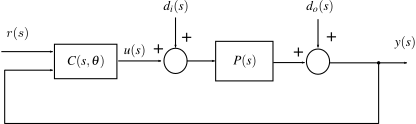
\includegraphics[width=0.8\columnwidth]{Ch4bloques}%pretex=\scriptsize,
	\caption{Feedback control loop.}% 
	\label{fig:bloques}%
\end{figure}
%
Figure~\ref{fig:bloques}, also called closed-loop control system, is designed to keep certain relationship between the process output $y(s)$ and the reference input $r(s)$. For such task, the difference between those signal is used to compute the control signal $u(s)$ needed in order to achieve $y(s)=r(s)$. 

In Figure.~\ref{fig:bloques}, $C(s,\bm{\theta})$ is the \gls{2dof} \gls{pid} controller with parameters:
\begin{equation*}
\bm{\theta}=\left[	\begin{tabular}{cccc} \gls{kp} & \gls{ti} & \gls{td} & \gls{beta}	\end{tabular}\right]^T
\end{equation*}
%
with \gls{kp} the proportional gain, \gls{ti} the integral time constant, \gls{td} is the derivative time constant, \gls{beta} the weight on the reference signal. \gls{plan} represents the controlled process, modeled as a \gls{soptd} plant, with a transfer function of the form:
\begin{equation}  %inclusión de ecuaciones
P(s) =  \frac{K e^{-Ls}}{(T s+1)(a T s+1)},
\label{eq:plantaX}
\end{equation}
%
where \gls{k}, \gls{l} and \gls{t}, correspond to the static gain, the time delay and main time constant respectively. The other pole of the system is represented with a time constant that is fraction of $T$, therefore $0 \leq a \leq 1$. \gls{di} represent the input disturbance while \gls{do} is the output disturbance.

%El diagrama de bloques de un controlador PI de dos grados de libertad se muestra en la Figura \ref{fig:controlador}. 
%
The relationship between the control signal, the reference and the process output is given by:
%
\begin{equation}  %inclusión de ecuaciones
\gls{u} = \gls{contr} \gls{r} - \gls{conty} \gls{y},
\label{us}
\end{equation}
%
where the part applied to the reference signal is given by:
%
\begin{equation}  %inclusión de ecuaciones
\gls{contr}=  \gls{kp}\left({\gls{beta} + \frac{1}{\gls{ti} s}+ \gls{gamma} \frac{\gls{td} s}{\gls{alpha} \gls{td} s +1}}\right),
\label{eq:cr}
\end{equation}
%
and the part applied to the process output is:
%
\begin{equation}  %inclusión de ecuaciones
\gls{conty}=  \gls{kp}\left({1 + \frac{1}{\gls{ti} s}+\frac{\gls{td} s}{\gls{alpha} \gls{td} s +1} }\right).
\label{eq:cy}
\end{equation}

It is common to set $\gls{alpha}=0.1$ and $\gls{gamma}=0$. For this reason, the controller parameter vector is give as $\gls{theta}=[\begin{tabular}{cccc} \gls{kp} & \gls{ti} & \gls{td} &\gls{beta} \end{tabular}]^T$. A detailed depiction of the controller transfer function is presented in 
\begin{figure}[tb]
	\centering
	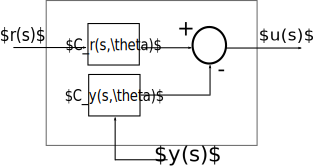
\includegraphics[width=0.6\columnwidth]{Ch4controlador}
	\caption{Representation of the \gls{2dof} controller.}
	\label{fig:Ch4controlador}
\end{figure}
%
Figure~\ref{fig:Ch4controlador}.

To simplify the analysis, the model of the controlled process is normalized:
%
\begin{equation*}
\hat{s}= Ts, \ \tau_0=  \displaystyle\frac{L}{T}, \ \tau_i=  \displaystyle\frac{T_i}{T}, \ \tau_d = \frac{T_d}{T}, \ \kappa_p= K_p K.
\end{equation*}  %inclusión de ecuaciones

Then the normalized parameters of the controller become $\bm{\theta}=\left[\kappa, \tau_i, \tau_d, \beta\right]^T$.
%
and the response of the controlled system is computed as: 
%%
\begin{equation} 
 y(\hat{s})= y_r(\hat{s}) + y_{di}(\hat{s}) + y_{do}(\hat{s}),
\label{ys}
\end{equation}
%
where $y_r(\hat{s})$, is the output response to a change in the setpoint $r(\hat{s})$, $y_{di}(\hat{s})$ is the response to a change in the input disturbance signal $d_i(s)$ and $y_{do}(\hat{s})$ is the response to a change in the ouput disturbace signal $d_o(s)$. From Figure~\ref{fig:bloques} and Figure~\ref{fig:Ch4controlador}, these signals can be computed as:
%
\begin{align*}
 y_r(\hat{s}) &= \frac{P(\hat{s}) C_r(\hat{s},\bm{\theta}) }{1 + P(\hat{s}) C_y(\hat{s},\bm{\theta})} r(\hat{s})\\
y_{di}(\hat{s}) &=  \frac{C_r(\hat{s},\bm{\theta})}{1 + P(\hat{s}) C_y(\hat{s},\bm{\theta})} d_i(\hat{s}) \\%
y_{do}(\hat{s}) &= \frac{1}{1 + P(\hat{s}) C_y(\hat{s},\bm{\theta})} {d_o(\hat{s})}
\label{ytot}
\end{align*}

%Dada \eqref{ys}, la respuesta de salida del lazo cerrado ante un cambio en el valor deseado puede ser ajustada a través del controlador de valor deseado $C_r(\hat{s},\theta)$, independientemente de cambios en la perturbación de entrada o en la de salida. Los parámetros de $C_r(\hat{s},\theta)$ y $C_y(\hat{s},\theta)$ son los mismos con un grado de libertad \cite{apuntescontrol}.

Robustness is an indication of the relative stability of the controlled system and it measure the ability of the controller to keep the closed loop stable despite the variation in the process dynamics. A metric of the degree of relative stability is the maximum sensitivity \gls{ms} given by:
%
\begin{equation}  %inclusión de ecuaciones
\gls{ms}=  \max_\omega \left\{ \frac{1}{\left |{1 + C_y(j\omega ) P(j\omega )}\right |}\right\} 
\label{Ms}
\end{equation}

The recommended value range is  $1.2\leq \gls{ms} \leq 2.0$.

As it is widely established, the controller tuning can be solved as a multi-objective optimization problem~\cite{Gambier2007}. One common indicator of performance, is the \gls{iae} given by:
%
\begin{equation}  %inclusión de ecuaciones
J(\bm{\theta})=\int_0^\infty \left |{e(t,\bm{\theta})}\right | dt.
\label{IAE}
\end{equation}

The error signal $e(t, \bm{\theta})$ it is calculated using:
%
\begin{equation}  %inclusión de ecuaciones
e(t,\bm{\theta})=r(t)-y(t,\bm{\theta}).
\label{error}
\end{equation}

When \eqref{IAE} is computed for a step change in the reference signal, the cost function becomes $J_r(\bm{\theta})$; for an input disturbance response, the function is defined as $J_{di}(\bm{\theta})$ and finally, for an output disturbance response, the cost function is named as $J_{do}(\bm{\theta})$.

When the output of the plant is disturbed only by the step change in $d_i(s)$, the error signal then becomes:
\begin{equation}  %inclusión de ecuaciones
e_d(t)=-y_{di}(t)
\label{per}.
\end{equation}

And then, the cost function $J_{di}(\bm{\theta})$ is computed as:
\begin{equation}  %inclusión de ecuaciones
J_{di}(\bm{\theta})= \int_0^\infty  \left |-{y_{di}(t,\bm{\theta})}\right | dt,
\label{perin}
\end{equation}

On the other hand, if the disturbance comes only from a step signal in $d_o(s)$, the cost function that has to be computed is $J_{do}(\bm{\theta})$ as:
%
\begin{equation}  %inclusión de ecuaciones
J_{do}(\bm{\theta})= \int_0^\infty  \left |-{y_{do}(t,\bm{\theta})}\right | dt.
\label{perout}
\end{equation}	
%

Finally, if the setpoint is the only source of disturbance for the plant, the corresponding cost function $J_r(\bm{\theta})$ is computed as:
\begin{equation}  %inclusión de ecuaciones
J_r(\bm{\theta})=\int_0^\infty \left |r(t)-y_r(t,\bm{\theta})\right | dt.
\label{eq:Jr}
\end{equation}
%

In general, it is not possible to optimize $\bm{\theta}$ for those three functions at the same time. Such impossible point where all the cost functions are optimal is called Utopia point, but optimizing one of them always produce a degradation in the other remaining functions. All the solutions that are closest to the utopia point, create the Pareto frontier which, if all cost functions are considered equal, are equally optimal. 

The problem of minimizing $J_r(\bm{\theta})$, $J_{di}(\bm{\theta})$ and $J_{do}(\bm{\theta})$ at the same time can be posed as a \gls{moo} problem. In addition, since in an industrial environment the robustness is very important, the obtained parameters are constrained to always satisfy  $\gls{ms} \leq M_{s,max}$, where $M_{s,max}$ is the allowed limit of the maximum sensitivity. The combined cost function (vector of cost functions) then becomes:
%
\begin{equation}  %inclusión de ecuaciones
\textbf{J}(\bm{\theta})=\left[J_{di}(\bm{\theta}), J_{do}(\bm{\theta}), J_{r}(\bm{\theta})\right]^T,
\label{eq:Jtotal}
\end{equation}
%
and solved by finding all possible optimal solutions of:
%
\begin{equation}  %inclusión de ecuaciones
\begin{gathered}
\textbf{J}(\bm{\theta}^*) = \min_{\bm{\theta}} \textbf{J}(\bm{\theta}),\\
\text{s.t.} \quad  M_s \leq M_{s,max}
\end{gathered}
\label{eq:probmoo}
\end{equation}

\textbf{To do: Expand more this part}